\documentclass[letterpaper,11pt]{article}
\usepackage{listings}
\usepackage[pdftex]{graphicx} 
\usepackage[utf8]{inputenc}
%\usepackage[english]{babel}
\usepackage{alltt}
\usepackage{color}
\usepackage{url}
\usepackage[T1]{fontenc}
\usepackage{float}
\usepackage{hyperref}
\usepackage{longtable}
\usepackage{caption}

\definecolor{dkgreen}{rgb}{0,0.6,0}
\definecolor{gray}{rgb}{0.5,0.5,0.5}
\definecolor{mauve}{rgb}{0.58,0,0.82}
\definecolor{codegreen}{rgb}{0,0.6,0}
\definecolor{codegray}{rgb}{0.5,0.5,0.5}
\definecolor{codepurple}{rgb}{0.58,0,0.82}
\definecolor{backcolour}{rgb}{0.95,0.95,0.92}

\addtolength{\textwidth}{4cm}
\addtolength{\hoffset}{-2cm}
\addtolength{\textheight}{4cm}
\addtolength{\voffset}{-2cm}

\lstdefinestyle{mystyle}{
    backgroundcolor=\color{backcolour},   
    commentstyle=\color{codegreen},
    keywordstyle=\color{magenta},
    numberstyle=\tiny\color{codegray},
    stringstyle=\color{codepurple},
    basicstyle=\footnotesize,
    breakatwhitespace=false,         
    breaklines=true,                 
    captionpos=b,                    
    keepspaces=true,                 
    numbers=left,                    
    numbersep=5pt,                  
    showspaces=false,                
    showstringspaces=false,
    showtabs=false,                  
    tabsize=2
}

\lstset{style=mystyle}

\lstset{
	basicstyle=\footnotesize,
	breaklines=true,
}

\title{Bibliography management: BibTeX}
\author{Share\LaTeX}

\begin{document}

\begin{titlepage}

\begin{center}

\Huge{Assignment 1}

\Large{CS834-F16:  Introduction to Information Retrieval}

\Large{Fall 2016}


\Large{Erika Siregar}

\vfill

% Bottom of the page
\Large{CS Department - Old Dominion University  \\ \today}


\end{center}

\end{titlepage}


\section*{Question 1.4}
\begin{verbatim}
List five web services or sites that you use that appear to use search, not
including web search engines. Describe the role of search for that service. 
Also describe whether the search is based on a database or grep style of matching,
or if the search is using some type of ranking.
\end{verbatim}

\subsection*{Answer}
Five web services that I use that appear to use search:
\begin{enumerate}
	\item \url{https://norfolk.craigslist.org/}
		\begin{itemize}
			\item \href{https://norfolk.craigslist.org/}{Craiglist} is a classified advertisements website with sections devoted to jobs, housing, personals, for sale, items wanted, services, community, gigs, résumés, and discussion forums \cite{craigslist}. User can type any query (something like `apartment near ODU' or `women bike') and \href{https://norfolk.craigslist.org/}{Craiglist} will return the search results ranked by their relevance or prices. 
		\end{itemize}
	\item \url{https://www.amazon.com/} 
		\begin{itemize}
			\item \href{https://www.amazon.com/}{Amazon} is the world's largest online retailer. It works in a similar way to \href{https://norfolk.craigslist.org/}{Craiglist}. User type a query of the thing that they want to buy online such as `waterproof women shoes'. \href{https://www.amazon.com/}{Amazon} responds to the query by showing the list of `waterproof women shoes' ranked by their relevance or prices. 
		\end{itemize}
	\item \url{https://www.usps.com/}
		\begin{itemize}
			\item The search role of this service is to track a package. A user can enter the tracking number and the system will return the current status and location of the package. 
			\item The search service that this system provides is clearly based on a database or grep style of matching. The system will take the number input by the user and find a matching record in the database. 
		\end{itemize}
	\item \url{http://www.urbandictionary.com/}
		\begin{itemize}
			\item The search role in \url{http://www.urbandictionary.com/} is to find definition of english slang words. The search results are ranked based on the number of votes that each definition has. The definition with the most votes will show up on the first order. 
		\end{itemize}
	\item \url{https://www.kayak.com/}
		\begin{itemize}
			\item \url{https://www.kayak.com/} is a travel site that aggregates all information from other travel sites and provides a recommendation for buying flight tickets. User can type the flight route and date and \href{https://www.kayak.com/}{Kayak} will give a suggestion about which ticket that user should buy. The search results are ranked based on the price, duration, and the number of stops. 
		\end{itemize}
\end{enumerate}
\noindent\makebox[\linewidth]{\rule{\textwidth}{0.4pt}}

\section*{Question 3.6}
\begin{verbatim}
How would you design a system to automatically enter data into web forms in order
to crawl deep Web pages? What measures would you use to make sure your crawler's
actions were not destructive (for instance, so that it does not add random blog
comments). 
\end{verbatim}

\subsection*{Answer:}
Web forms is one category of the deep web, which can only be accessed by filling out web forms. We cannot obtain the data if there is no human interaction with the web forms. In this case, the challenge is \textit{``forms are designed to be handled by human, so how can we automate it?"}.\\
The simplest solution will be submitting the combination of all possible field values in cartesian product. However, this solution is not feasible when the number of fields and possible values are large. Thus, the goal is not to find all possible values, but to select a subset of values so as to minimize the number of submissions and maximize the coverage (retrieve more distinct data behind the form) \cite{kantorski2012automatic}. 
Kantorski \cite{Kantorski:2015:AFH:2783888.2783898} conducted a survey to compare 15 approaches for handling automatic web form filling. All these methods have a common thread regarding how they address the problem of web form filling. They always have to deal with: 
\begin{enumerate}
	\item form detection: determine the field and domain of the form.
	\item initial value generation:  select words from the initial page, where the form is located
	\item value generation: iteratively submitting queries using values obtained in previous iterations. 
\end{enumerate}

One method that is really interesting for me is the one proposed by Barbosa and Freire \cite{barbosa2010siphoning} about using keywords to siphon the hidden data. Instead of blindly issuing queries, they proposed a sampling-based approach to discover words that result in high coverage. The intuition is that words in the actual database or document collection are more likely to result in higher coverage than randomly selected words. Barbosa and Freire \cite{barbosa2010siphoning} come up with the idea of using sampling and probing to generate high-coverage query. Sampling is used to find high-frequency keywords (the candidate keywords). These candidate keywords will be combined into a query and used in site probing to determine the query cardinality. Queries with low cardinality are deemed not effective and removed from the database. Figure \ref{fig:sampling_probing} summarize the algorithm. 

\begin{figure}[H]
\fbox{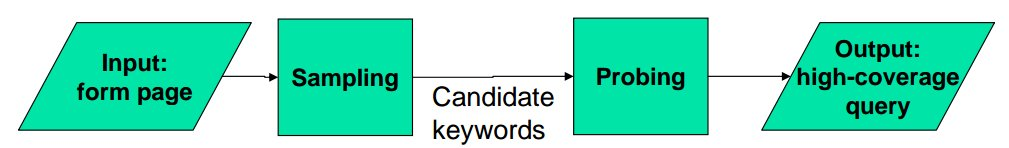
\includegraphics[width=\textwidth, height=\textheight, keepaspectratio]{sampling_probing}}
\centering
\caption{Sampling and probing to generate high-coverage query. Adapted from  \url{https://vgc.poly.edu/~juliana/pub/sbbd2004-talk.pdf}}
\label{fig:sampling_probing}
\end{figure}

Furthermore, figure \ref{fig:sampling} illustrates the processes that happen in `sampling'. Basically, sampling is a process to turn the input `terms in the form page' into the output `candidate (high-frequency) keywords'. Candidate keywords are produced by iteratively submitting queries using values obtained in previous iterations based on term frequency. 

\begin{figure}[H]
	\fbox{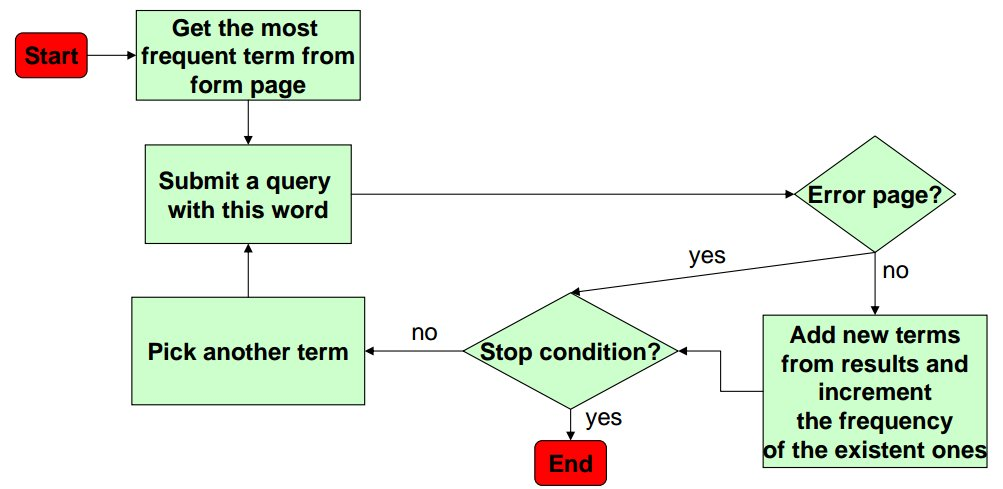
\includegraphics[width=\textwidth, height=\textheight, keepaspectratio]{sampling}}
	\centering
	\caption{Sampling algorithm for building candidate keywords. Adapted from \url{https://vgc.poly.edu/~juliana/pub/sbbd2004-talk.pdf}}
	\label{fig:sampling}
\end{figure}

The response page for a query may contain information that is not relevant to the actual query (e.g. ads, navigation bars) that is not part of the site. This information may negatively impact the keyword selection process. Hence, it must be removed before selecting the candidate words. We also have to consider doing additional techniques such as removing stop words and stemming. \\
To ensure that our design is not destructive, we have to send only GET requests. By using GET method, we can guarantee that the crawler will not inadvertently post something such as posting blog comments or order a product. Since the crawlwer's job is to retrieve data that is already exists on the server (not to tell something to the server), a crawler should use GET method and avoid POST method. Also, filtering away form contains login/personal information (user-name, password, etc.) will be a good idea. It could help to make sure that the query that we submit does not create new documents on the server side. 

\noindent\makebox[\linewidth]{\rule{\textwidth}{0.4pt}}

\section*{Question 3.9}
\begin{verbatim}
Write a simple single-threaded web crawler. Starting from a single input URL
(perhaps a professor’s web page), the crawler should download a page and then
wait at least five seconds before downloading the next page. Your program should
find other pages to crawl by parsing link tags found in previously crawled
documents.
\end{verbatim}

\subsection*{Answer}
Web crawler is a program that find and download web pages automatically. A web crawler is designed to follow the links on web pages to discover and download new pages. This program runs recursively, meaning that it will repeat itself everytime it download a new page. This process continues until the crawler either runs out of disk space to store pages or runs out of useful links to add to the request queue  \cite{Croft:2009:SEI:1516224}. For the purpose of this assignment only, the user will be asked to enter the maximum number of recursive calls for the crawling process. 
To create the web crawler program, I modified the program that I made in web science class about extracting 1000 links from Twitter. Therefore, I once again utilize useful python libraries named Beautiful Soup \cite{bs4} and Requests \cite{requests}. 

The web crawler program can be summarize into this algorithm:
\begin{enumerate}
	\item Capture the keyboard input. User will be prompted to enter :
		\begin{itemize}
			\item The initial URI (the seed).
			\item The number of recursive calls (the level) that they want to make.
			\item The path to output folder
		\end{itemize}
	\item Strip the seed URI.
	\item Crawl the seed URI (follow the link and download the page) using library `Requests'.
	\item If the URI's status code is 200:
		\begin{itemize}
			\item Parse HTML with beautiful soup.
			\item Find all <a> tags.
			\item Get href attribute from tag <a>. 
			\item Sometimes url in tag <a> is not a full url (e.g: <a href="/folder/a.html">...</a>). So, we have to add the schema and host to create an absolute URI. 
			\item Add these new found URIs to the frontier.
		\end{itemize}  
	\item While our current level is less than depth (level < depth), then repeat the crawling process again using the URIs in the frontier. 
	\item Wait for 5 seconds before downloading the next page. 
	\item The outputs of this program are the downloaded html page and the list of extracted links. 
\end{enumerate}

Listing \ref{lst:web-crawler} shows the complete code for the web crawler. 

\begin{lstlisting}[language=python, caption={Simple single-threaded web crawler}, label={lst:web-crawler}]

#!/usr/bin/python

import hashlib
import os
from urlparse import urljoin

import errno
import requests as requests
import time
from bs4 import BeautifulSoup
from requests.exceptions import InvalidSchema


def open_url(level, idx, url, outdir):
    url = url.strip()

    # Hashing URL as a output file
    outfile = os.path.join(outdir, hashlib.md5(url).hexdigest() + '.html')
    listfile = os.path.join(outdir, 'urls.csv')

    # Crawl URL with requests, methods GET
    print('Debug : {}.{} Opening URL {}'.format(level+1, idx+1, url))

    try:
        resp = requests.get(url)

        # Process only if status code 200
        if resp.status_code == 200:
            print('Debug : {}.{} URL {} is opened'.format(level+1, idx+1, url))

            html = resp.text

            # Save html to outfile
            with open(outfile, 'w') as of:
                of.write(html.encode('utf-8'))
                print('Debug : {} is saved into {}'.format(url, outfile))

            # Save url to list
            with open(listfile, 'a') as f:
                f.write(url + '\n')

            # Parse HTML with beautiful soup
            soup = BeautifulSoup(html, 'html.parser')
            # Find all anchors, <a> tag
            links = soup.find_all('a')

            # Get href attribute from tag <a>
            hrefs = []
            for link in links:
                href = link.get('href')

                # Make url absolute
                # Sometimes url in tag <a> is not a full url, without schema and host
                # e.g: <a href="/folder/a.html">...</a>
                href = urljoin(url, href)

                hrefs.append(href)

            return hrefs
        else:
            print('Debug : {}.{} Cannot open URL {}, Status code: {}'.format(level+1, idx+1, url,
                                                                             resp.status_code))
    except:
        pass


# Capture input from keyboard
url = raw_input("Enter a URL: ")

depth = raw_input("Enter crawl depth or level: ")
depth = int(depth)

outdir = raw_input("Enter output directory: ")
# Make directory if not exists
try:
    os.makedirs(outdir)
except OSError as exc:
    if exc.errno != errno.EEXIST:
        raise

links = [url, ]

level = -1
while level < depth:
    # Prepare childre_links to save newly founded links
    children_links = []
    for idx, link in enumerate(links):
        # open_url will return new list of links founded in link
        new_links = open_url(level, idx, link, outdir)
        if new_links:
            print('Debug : Found {} links'.format(len(new_links)))
            children_links = children_links + new_links

        # Sleep for 5 seconds
        print('Debug : Sleep for 5 seconds')
        time.sleep(5)

    # After all links are processed, set links with children_links and increase level
    links = children_links
    level += 1


\end{lstlisting}

Figure \ref{fig:crawler} shows the crawling process that happens when we run the crawler using  \url{http://www.cs.odu.edu/~mln/} as the seed and the number of recursive calls = 1. Figure \ref{fig:url} shows the extracted links resulted from the crawling process. 


\begin{figure}[H]

\fbox{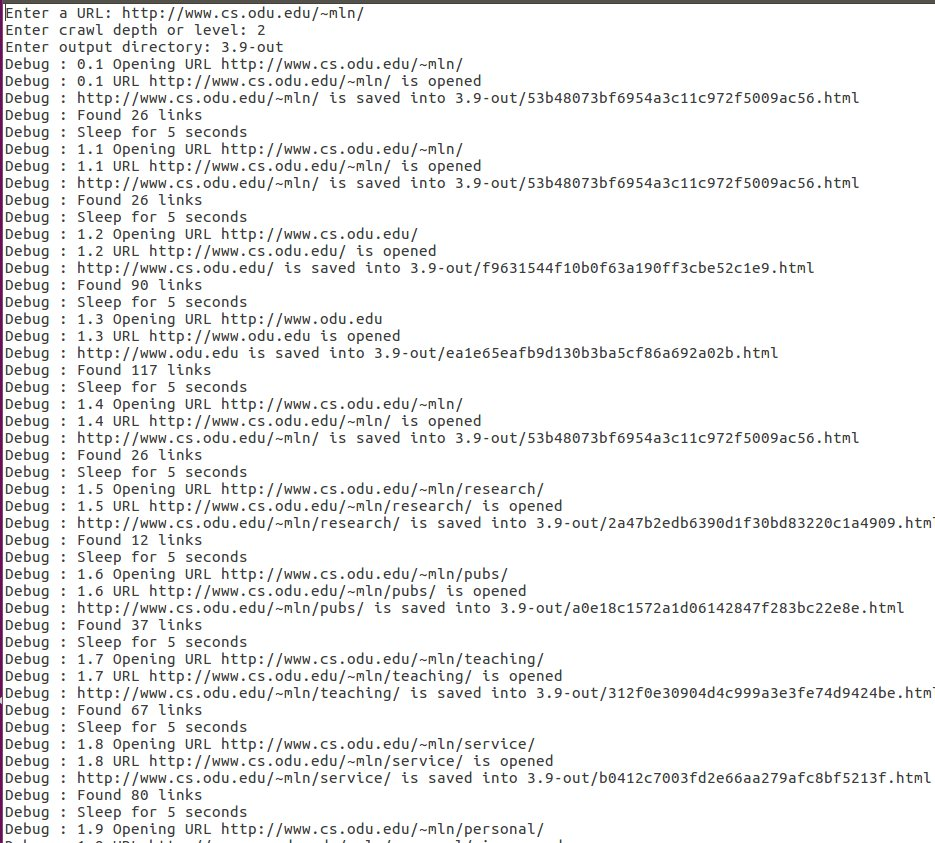
\includegraphics[width=\textwidth, height=\textheight, keepaspectratio]{crawling_process}}

\centering

\caption{The crawling process}

\label{fig:crawler}

\end{figure} 

\begin{figure}[H]

\fbox{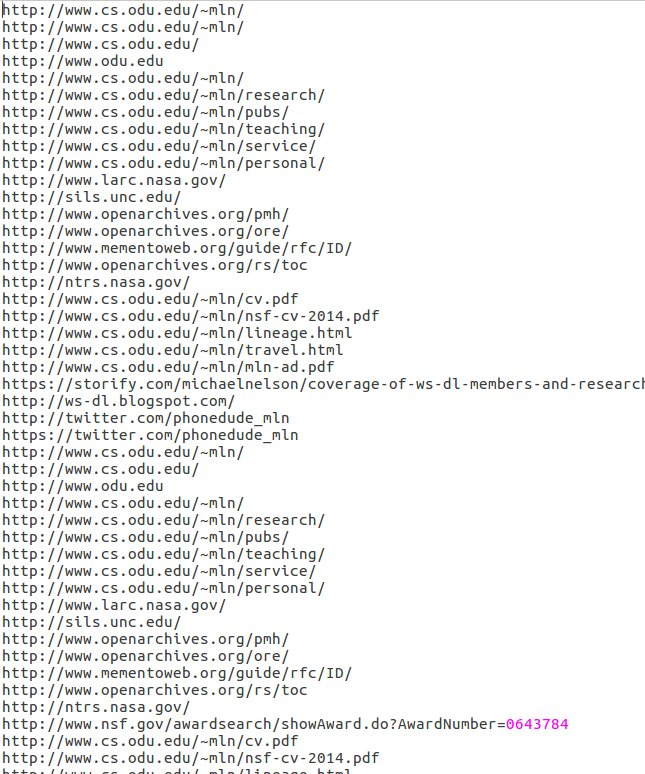
\includegraphics[width=\textwidth, height=\textheight, keepaspectratio]{url}}

\centering

\caption{The Extracted Link from \url{http://www.cs.odu.edu/~mln/}}

\label{fig:url}

\end{figure} 

All outputs resulted from the crawling process (including the downloaded html pages and the list of extracted links) are uploaded to github under directory assignments/a1/crawling\_output. 

\noindent\makebox[\linewidth]{\rule{\textwidth}{0.4pt}}

\section*{Question 3.12}
\begin{verbatim}
Design a compression algorithm that compresses HTML tags. Your algorithm should
detect tags in an HTML file and replace them with a code of your own design that
is smaller than the tag itself. Write an encoder and decoder program.
\end{verbatim}

\subsection*{Answer}
To solve this problem, the first thing that we have to do is to identify all tags in the input HTML file. The tags in HTML file can be distinguished into 2 categories: `start\_tag' and `end\_tag'. We can take advantage of HTMLParser \cite{txt-compression}, a python library for parsing text files formatted in HTML (HyperText Mark-up Language) and XHTML. HTMLParser provides complete functions to handle start\_tag, end\_tag, and data. For this assignment, I will create two programs: the encoder and the decoder. \\
Here are the general algorithm to tackle this problem. We start with creating the encoder program: 
\begin{enumerate}
	\item Create a class \textit{HTMLEncoder} which is an extension of \textit{HTMLParser}. 
	\item Scan the input HTML file. 
	\item Parse the HTML file and identify all tags (start\_tag and end\_tag) and data in the HTML file. We do this using `feed' function from HTMLParser. 
	\item Store the list of the tags into an array. 
	\item Compress the tags by replacing them with character smaller than the tag itself. Use the character that represents the tag index in the array. For example: 
	\begin{itemize}
		\item if index = 0, then char = a.
		\item if index = 1, then char = b. \\
		etc.
	\end{itemize}
	\item Concatenate the new compressed tags and the data and store them in a string named `minified\_html'.
	\item Create a HTML comment contains the mapping relation between the original tags and the compressed tags. Append this comment to the string `minified\_html'. 
	\item Write down the `minified\_html' into a file. 
\end{enumerate}
	
For the decoder program, we basically do the similar things as we did in the encoder program, but in reverse order:
\begin{enumerate}
	\item Read the comment in `minified\_html' that contains the mapping between the compressed tags and the original tags. 
	\item Parsing the compressed HTML file to identify all compressed tags in that HTML file. 
	\item Replace the compressed tags with the original tags. 
\end{enumerate}
	
Figure \ref{fig:compressedTag} shows the terminal output for the `Compress HTML Tags' program. 

\begin{figure}[H]

	\fbox{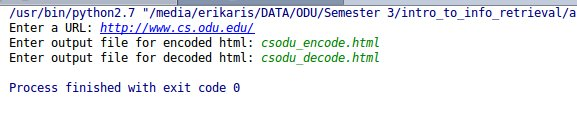
\includegraphics[width=\textwidth, height=\textheight, keepaspectratio]{compressedTag}}

	\centering

	\caption{Terminal output for the `Compress HTML tags' program}

	\label{fig:compressedTag}

\end{figure}

The complete encoder and decoder code for HTML-tag compressing can be seen in listing \ref{lst:tag-compressing-encoder} and listing \ref{lst:tag-compressing-decoder}, respectively.

\begin{lstlisting}[language=python, caption={Encoder for HTML-tag Compressing }, label={lst:tag-compressing-encoder}]
 
import json
import string
from HTMLParser import HTMLParser

import htmlmin as htmlmin
import requests


# HTMLEncoder is extent of HTMLParser
class HTMLEncoder(HTMLParser):
    _tags = []

    def handle_starttag(self, tag, attrs):
        # Append to array, with type 'starttag'
        self._tags.append(((tag, attrs), 'starttag'))

    def handle_endtag(self, tag):
        # Append to array, with type 'endtag'
        self._tags.append((tag, 'endtag'))

    def handle_data(self, data):
        # Append to array, with type 'data'
        self._tags.append((data, 'data'))

    def make_chars(self, number):
        num_char = int(number/len(string.lowercase))
        rem = number - (num_char * len(string.lowercase))

        chars = ''.join([string.lowercase[len(string.lowercase)-1] for i in range(0,num_char)]) + \
                string.lowercase[rem]

        return chars

    def encode(self, html):
        # Process normal html with HTMLParser
        self.feed(html)
        self.close()

        # After parsing is done, process array _tags
        tag_list = []
        minified_html = ''
        for data, type in self._tags:
            if type == 'starttag':
                (tag, attrs) = data

                if not tag in tag_list:
                    tag_list.append(tag)

                # Process attrs of tag, e.g:
                # [('href', 'http://...'), ('title', 'Some link')] become
                # <a href='http://...' title='Some link'>
                str_attrs = ' '.join(['{}="{}"'.format(name, val) for name, val in attrs])

                # Append encoded tag and it's attrs into var html
                encoded_tag = self.make_chars(tag_list.index(tag))
                minified_html += '<{}{}>'.format(
                    encoded_tag, (' ' if str_attrs else '') + str_attrs
                )
            elif type == 'endtag':
                # Append encoded end-tag into var html
                encoded_tag = self.make_chars(tag_list.index(tag))
                minified_html += '</{}>'.format(encoded_tag)
            elif type == 'data':
                # Append data into var html
                minified_html += data

        # Process json of definition as a comment
        definitions = '<!--{}-->'.format(
            json.dumps({ self.make_chars(key): val for key, val in enumerate(tag_list) })
        )

        # Return definition and minified html
        return definitions + minified_html

\end{lstlisting}	

\begin{lstlisting}[language=python, caption={Decoder for HTML-tag Compressing }, label={lst:tag-compressing-decoder}]

decoder# HTMLDecoder is extent of HTMLParser
class HTMLDecoder(HTMLParser):
    _tag_map = {}
    _tags = []

    def handle_comment(self, data):
        # Comment contains mapper of html tags
        original_tag_map = json.loads(data)

        # There are more than one comments
        # Process only comment type json
        if type(original_tag_map) == dict:
            self._tag_map = original_tag_map

    def handle_starttag(self, tag, attrs):
        # Append to array, with type 'starttag'
        self._tags.append(((tag, attrs), 'starttag'))

    def handle_endtag(self, tag):
        # Append to array, with type 'endtag'
        self._tags.append((tag, 'endtag'))

    def handle_data(self, data):
        # Append to array, with type 'data'
        self._tags.append((data, 'data'))

    def decode(self, enc_html):
        # Process normal html with HTMLParser
        self.feed(enc_html)
        self.close()

        # After parsing is done, process array _tags
        html = ''
        for data, type in self._tags:
            if type == 'starttag':
                (tag, attrs) = data

                # Process attrs of tag, e.g:
                # [('href', 'http://...'), ('title', 'Some link')] become
                # <a href='http://...' title='Some link'>
                str_attrs = ' '.join(['{}="{}"'.format(name, val) for name, val in attrs])

                # Append decoded tag and it's attrs into var html
                html += '<{}{}>'.format(
                    self._tag_map[tag],
                    (' ' if str_attrs else '') + str_attrs
                )
            elif type == 'endtag':
                # Append decoded end-tag into var html
                html += '</{}>'.format(self._tag_map[tag])
            elif type =='data':
                # Append data into var html
                html += data

        return html
\end{lstlisting}

I tested the encoder and decoder program using URI: \url{http://www.cs.odu.edu/}. Figure \ref{fig:csodu_encode_jpg} shows the HTML output for tag-compressed \url{http://www.cs.odu.edu/} and figure \ref{fig:csodu_decode_jpg} shows the HTML file after being decoded to its original tags. 

\begin{figure}[H]
	\fbox{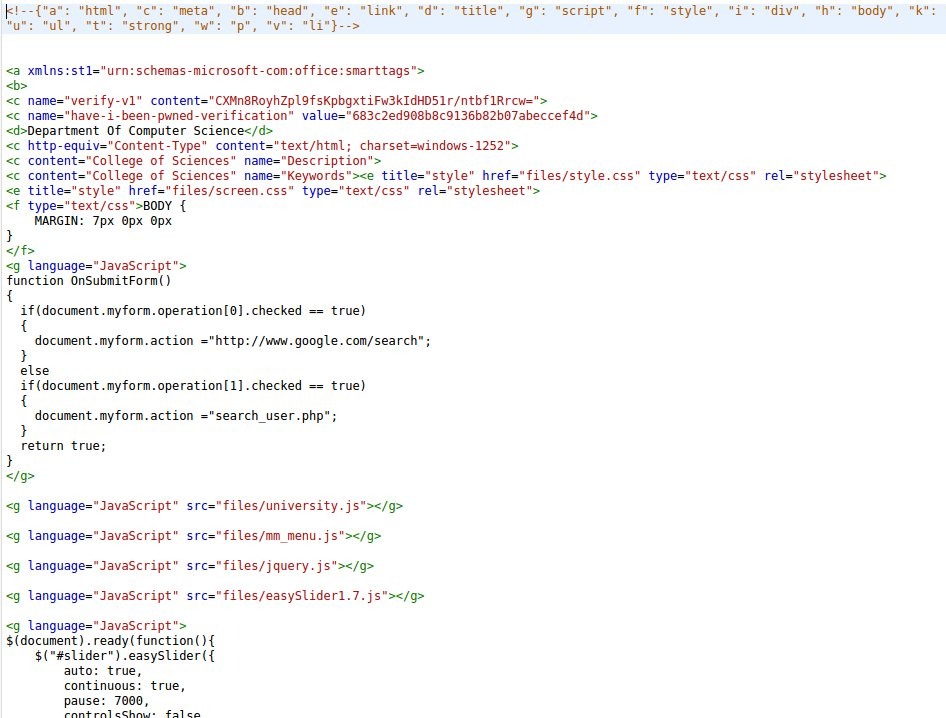
\includegraphics[width=\textwidth, height=\textheight, keepaspectratio]{csodu_encode_jpg}}
	\centering
	\caption{Encoding output (tag-compressed) for \url{http://www.cs.odu.edu/}}
	\label{fig:csodu_encode_jpg}
\end{figure}

\begin{figure}[H]
	\fbox{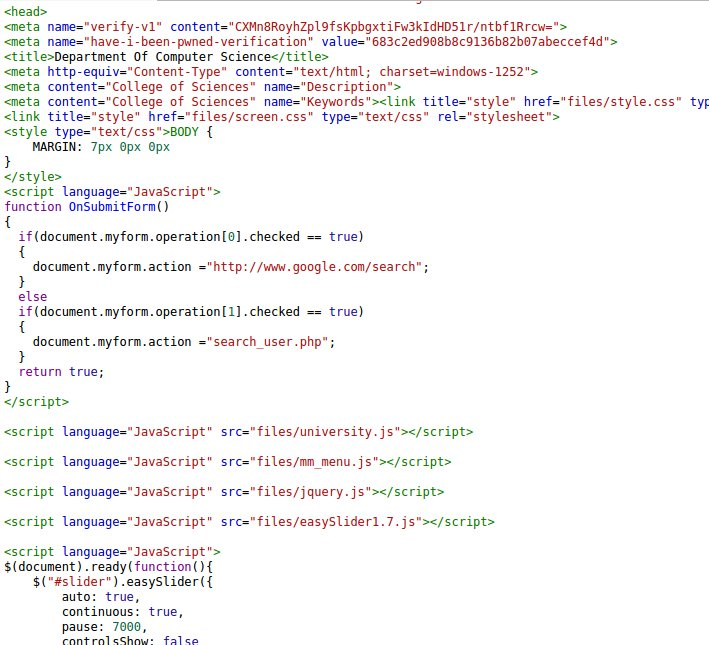
\includegraphics[width=\textwidth, height=\textheight, keepaspectratio]{csodu_decode_jpg}}
	\centering
	\caption{Decoding output (tag-uncompressed) for \url{http://www.cs.odu.edu/}}
	\label{fig:csodu_decode_jpg}
\end{figure}

\noindent\makebox[\linewidth]{\rule{\textwidth}{0.4pt}}


\section*{Question 3.16}
\begin{verbatim}
Give a high-level outline of an algorithm that would use the DOM structure to
identify content information in a web page. In particular, describe heuristics
you would use to identify content and non-content elements of the structure.
\end{verbatim}

\subsection*{Answer}

According to Lopez et al \cite{lopez2012using}, content extraction could be done using CNR (Chars-nodes ratio) algorithm, which shows the relation between text content and tags content of each node in the DOM tree. Figure \ provides an illustration of the DOM Tree for content extraction. CNR considers nodes as blocks where the internal information is grouped and indivisible using the DOM structure. CNR of an internal node takes into account all the texts and tags included in its descendants. 

\begin{figure}[H]
	\fbox{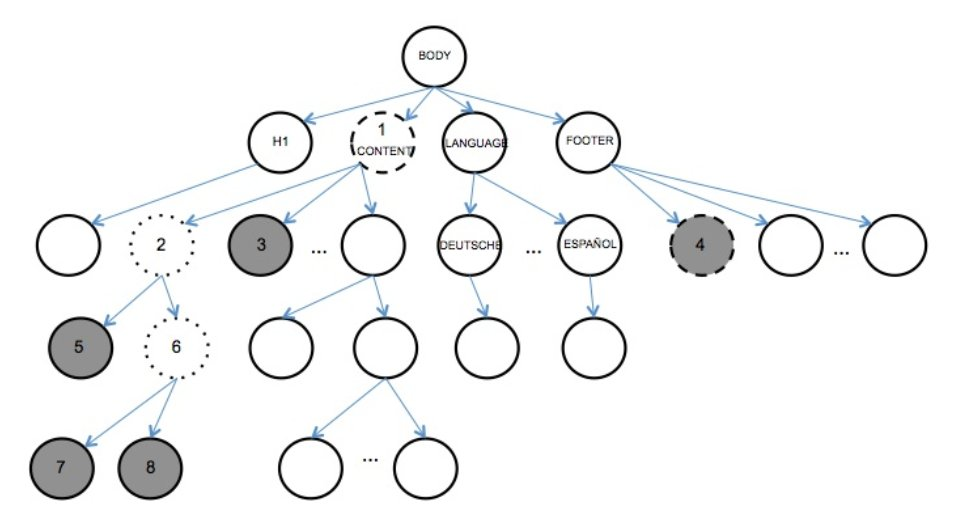
\includegraphics[width=\textwidth, height=\textheight, keepaspectratio]{dom_tree}}

	\centering

	\caption{DOM Tree representation for content extraction. Adapted from \cite{lopez2012using}}

	\label{fig:dom_tree}
\end{figure}

Steps for content extraction:
\begin{enumerate}
	\item Compute the CNR for each node in the DOM tree.\\
	 It ignores irrelevant code that should not be counted as text called “nonContentNode”, for instance, nodes without text (e.g., img), nodes mainly used for menus (e.g., nav and a) and irrelevant nodes (e.g., script, video and svg). Computation of CNRs is done with a cumulative and recursive process that explores the DOM tree counting the text and descendants of each node. This step recursively obtains the CNR of each node starting at the root node of the DOM tree. At each node it adds three new attributes to the node with the computed weight (weight), the number of characters it contains (textLength), and the CNR (CNR). Figure \ref{fig:dom_extract_alg1} shows the algorithm to compute CNR. 
	\item \label{en:step-2} Select those nodes with a higher CNR.
	\item Starting from step \ref{en:step-2}, traverse the DOM tree bottom-up to find the best container nodes (e.g., tables, divs, etc.) that, roughly, contain as more relevant text as possible and less nodes as possible. Each of these container nodes represents an HTML block.\\
	In this step, it removes all the nodes in the set that are descendant of other nodes in the set. Then, it proceeds bottom-up in the tree by discarding brother nodes and collecting their parent until a fix point is reached. This process produces a final set of nodes that represent blocks in the webpage. Figure \ref{fig:dom_extract_alg2} shows the algorithm to identify main content blocks. 
	\item Choose the block with more relevant content. The final block contains more text (in the subtree rooted at that node).
\end{enumerate}

\begin{figure}[H]
	\fbox{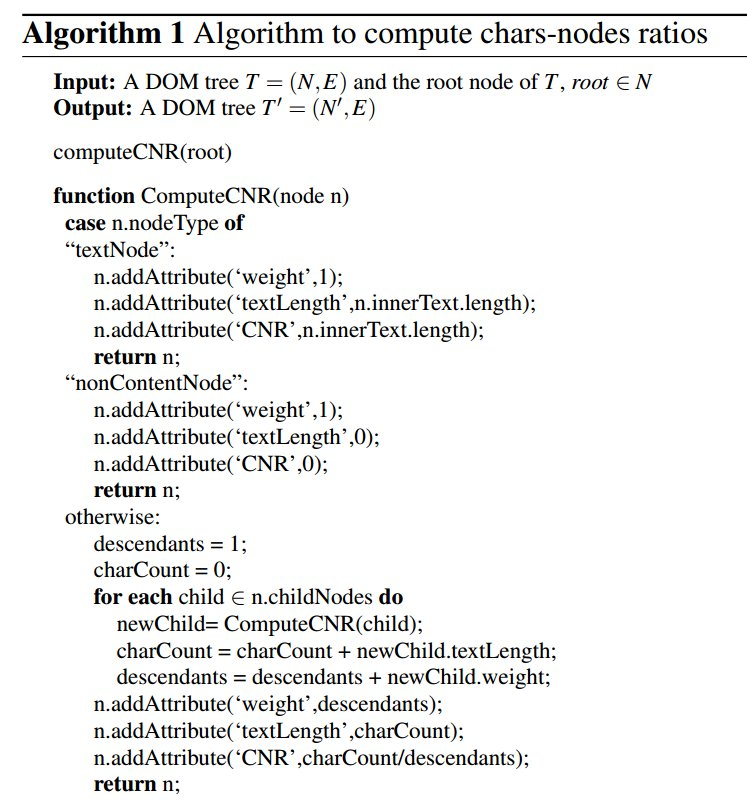
\includegraphics[scale=0.6]{dom_extract_alg1}}

	\centering

	\caption{Algorithm to compute CNR. Adapted from \cite{lopez2012using}}

	\label{fig:dom_extract_alg1}
\end{figure}


\begin{figure}[H]
	\fbox{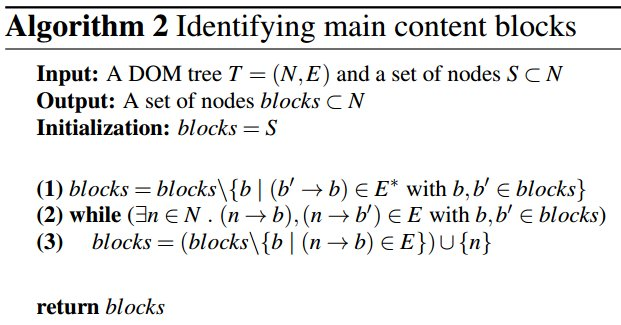
\includegraphics[scale=0.6]{dom_extract_alg2}}

	\centering

	\caption{Algorithm to identify main content blocks. Adapted from \cite{lopez2012using}}

	\label{fig:dom_extract_alg2}
\end{figure}

\medskip

\bibliographystyle{unsrt}%Used BibTeX style is unsrt
\bibliography{biblio}

\end{document}
